\documentclass[conference, a4paper, mongolian]{myIEEEtran}
%\usepackage[T2A]{fontenc}
\usepackage[utf8]{inputenc}
\usepackage{babel}
\usepackage{cite}
\usepackage[caption=false]{subfig}
\usepackage{url}
\usepackage{hyperref}
\hypersetup{
    colorlinks=true,
    linkcolor=[rgb]{0, 0.356, 0.509},
    urlcolor=[rgb]{0, 0.356, 0.509},
    citecolor=[rgb]{0, 0.356, 0.509},    
    pdftitle={Master Thesis},
    pdfauthor={Enkh-Erdene Jargalsaikhan},
}

%\usepackage{substitutefont}
%
%\substitutefont{T2A}{\familydefault}{Tempora-TLF}
%\makeatletter
%\input{t2atempora-tlf.fd}
%\DeclareFontShape{T2A}{Tempora-TLF}{m}{sc}{
%      <-> ssub * Tempora-TLF/m/n
%}{}

\renewcommand{\sfdefault}{cmss}
\renewcommand{\rmdefault}{cmr}
\renewcommand{\ttdefault}{cmt}

\def\IEEEkeywordsname{Түлхүүр үгс}

\IEEEoverridecommandlockouts

\usepackage{amsmath,amssymb,amsfonts}
\usepackage{algorithmic}
\usepackage{graphicx}
\usepackage{textcomp}
\usepackage{xcolor}
\def\BibTeX{{\rm B\kern-.05em{\sc i\kern-.025em b}\kern-.08em
    T\kern-.1667em\lower.7ex\hbox{E}\kern-.125emX}}

\begin{document}
\renewcommand{\abstractname}{Хураангуй}

\title {МУИС-ийн сургалттай холбоотой \\ онтологи үүсгэх нь}

\author{
	\IEEEauthorblockN{Ж. Энх-Эрдэнэ}
	\IEEEauthorblockA{
		Мэдээлэл, Компьютерийн Ухааны Тэнхим \\
		ХШУИС, Монгол Улсын Их Сургууль \\
		Улаанбаатар, Монгол улс
	}
	\and
	\IEEEauthorblockN{Г. Амарсанаа}
	\IEEEauthorblockA{
		Мэдээлэл, Компьютерийн Ухааны Тэнхим \\
		ХШУИС, Монгол Улсын Их Сургууль \\
		Улаанбаатар, Монгол улс
	}
}

\maketitle
\thispagestyle{plain}
\pagestyle{plain}

\begin{abstract}
Энэхүү өгүүлэлд МУИС-ийн сургалтын үйл ажиллагааны талаарх ойлголтуудыг багтаасан Монгол хэл дээрх онтологийн бүтцийг боловсруулж,  холбогдох мэдээллийг өргөн хүрээнд хайх боломж бүхий семантик аппликейшны ерөнхий шаардлагыг тодорхойлсон. Тус судалгаа нь цаашид хөгжүүлэх боломжтой анхан шатны загвар онтологи бий болгоход чиглэгдсэн бөгөөд тухайн чиглэлийн зөвхөн суурь ойлголтуудыг авч үзсэн болно.\\
\end{abstract}

\begin{IEEEkeywords}
семантик вэб; онтологи
\end{IEEEkeywords}
%
\section{Удиртгал}
%
Өнөөгийн вэб технологийн дараагийн үе шат болох семантик вэб нь онлайн орчинд хадгалагдах асар их хэмжээний мэдээллийн нөөцийг ухаалгаар удирдаж ашиглах боломжийг олгоно \cite{bib:1}. Семантик вэб технологийг бодитоор нэвтрүүлэхийн тулд аливаа мэдлэг мэдээллийг хэрэглэгдэх хүрээ, ерөнхий онцлогоос нь хамааруулан нэгтгэж хоорондын харилцаа холбоог дэлгэрэнгүй илэрхийлсэн багц ойлголт болох онтологиудыг үүсгэх шаардлагатай \cite{bib:2}.

Олон төрлийн багц мэдлэгүүдийг ийнхүү онтологи болгон бүтэцлэснээр ялгаатай ойлголтуудыг нэгтгэж зохицуулах боломж бүрдэнэ. Тухайлбал боловсролын салбар, түүний хамгийн чухал хэсэг их сургуульд хамаарах мэдлэг, мэдээллийг ерөнхийлөн цэгцэлж онтологи болгон хэлбэржүүлснээр семантик вэбийн үндсэн зорилго шаардлагад тодорхой хэмжээнд нэмэр болж буй хэрэг юм.

Хэдий их сургуультай холбоотой ойлголтыг илэрхийлсэн онтологи цөөнгүй хөгжүүлэгдсэн ч Монгол хэл дээр бус, мөн тухайн сургууль, бусад орчин нөхцөлөөс шалтгаалж Монгол Улсын Их Сургууль (МУИС)-ийн онцлогт нийцүүлэн ашиглахад бүрэн зохицолгүй зэрэг асуудал тулгарсаар байна. Энэ ажлын зорилго нь МУИС-ийн хичээл, сургалтад хамаарах ойлголтуудыг Монгол хэлээр илэрхийлсэн анхны (бидэнд мэдэгдэж буйгаар) онтологийг байгуулах юм.

Уг өгүүллийн дараагийн бүлэгт их сургуулийн айн (domain) онтологи үүсгэхтэй холбоотой өмнө хийгдсэн судалгааны ажлуудыг авч үзсэн бол 3-р бүлэгт өөрсдийн онтологийн загвар зохиомжийг, 4 болон 5-р бүлэгт ажлын үр дүн, дүгнэлтийг тусгалаа.
%
\section{Холбоотой ажлууд}
%
Prot\'eg\'e \footnote{\url{https://protege.stanford.edu}} хэрэгсэл ашиглан их сургуулийн онтологи байгуулах \cite{bib:3}, их сургуулийн онтологи үүсгэх ерөнхий аргачлал \cite{bib:4}, семантик вэбд зориулсан загвар хэл SHOE\footnote{Simple HTML Ontology Extensions} \cite{bib:5} зэрэг ажлууд нь их сургуулийн айн онтологи бүтээх асуудлыг хөнджээ.

Prot\'eg\'e хэрэгсэл ашиглан их сургуулийн онтологи байгуулах ажлаар Энэтхэгийн ``Ражив Гандийн нэрэмжит Техникийн Их Сургууль``-ийн онтологийг үүсгэх талаар авч үзсэн байна. Ингэхдээ харгалзах онтологийн дотоод бүтцийг бус prot\'eg\'e хэрэгслийн ач холбогдол, хэрэгжүүлэлтийн алхмуудыг голчлон анхаарч судалжээ.

Их сургуулийн онтологи үүсгэх ерөнхий аргачлалын талаарх судалгааны ажилд багш, оюутны оролцоогоор их сургуулийн аливаа хичээлийн нарийн мэдлэг шаардах ойлголтуудыг тодорхойлуулах, цаашлаад онтологи үүсгэх зорилго бүхий тусгай хичээлээр дамжуулж их сургуулийн айн онтологи байгуулах санааг дэвшүүлсэн байна.

Семантик вэбийн SHOE загвар хэлийг ашиглан онтологи байгуулах \cite{bib:6} ажилд их сургуулийн судалгаа, судалгааны товхимол, оюутан, тэнхим, салбар сургуулиуд зэрэг нэгжүүдийг хамарсан онтологийг үүсгэсэн. Үүнд хичээл болон хичээлийн төрлүүд, хөтөлбөр, үнэлгээ гэх мэт сургалттай холбоотой нэгж ойлголтуудыг авч үзээгүй ба өмнөх бүлэгт дурдсанчлан МУИС-ийн бүтэц, онцлогийг бүрэн илэрхийлэх онтологи биш гэдэг нь олон талаар харагдсан.

Дээрх ажлууд нь бүгд Англи хэл дээр, мөн шууд нутагшуулж ашиглах боломж хомс байгаа нь МУИС-д зориулсан Монгол хэл дээр онтологи үүсгэх асуудал чухал ач холбогдолтойг харуулж байна.
%
\section{Онтологи загварчлал}
%
\begin{figure*}[t]
	\centering
	\subfloat[Классуудын шатлал]{
		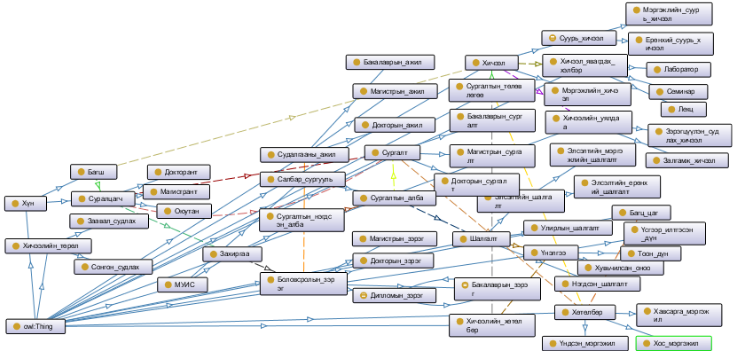
\includegraphics[width=0.8\linewidth]{figures/class_hierarchy}
		\label{figure:class_hierarchy}
	} \\
	\subfloat[Хамаарлын нэгжүүд]{
		\includegraphics[width=0.2\linewidth]{figures/object_hierarchy}
		\label{figure:object_hierarchy}
	}
	\hfil
	\subfloat[Төрлийн нэгжүүд]{
		\includegraphics[width=0.2\linewidth]{figures/data_hierarchy}
		\label{figure:data_hierarchy}
	}
	\caption{Үүсгэсэн онтологийн ерөнхий бүтэц.}
	\label{figure:ontology}
\end{figure*}
%
Бид өөрсдийн онтологийг \cite{bib:7}-д санал болгосон ``зорилтот загвар`` (purpose-oriented model) нэртэй онтологи үүсгэх арга зарчим дээр тулгуурлан байгуулна. Энэхүү арга нь:
%
\begin{enumerate}
	\item Онтологийн зорилго, ашиглах хүрээг тодорхойлох,
	\item Ижил төстэй нөөцүүдийг олж тогтоох,
	\item Онтологид хамаарах чухал ойлголт, нөхцөлүүдийг судалж илрүүлэх,
	\item Классууд, классуудын ангилал, шинж чанар, харилцаа холбоог зохиомжлох,
	\item Баримт, тохиолдлуудыг оруулж турших
\end{enumerate}
зэрэг алхмуудаас тогтоно.
%
\subsection{Aй}
%
Эхлээд үүсгэх гэж буй онтологийн айг илэрхий болгохын зэрэгцээ бусад нөөц (resource)-ийг аль болох дахин ашиглах хэрэгтэй. МУИС-ийн сургалтын үйл ажиллагаа нь бидний онтологийн ай юм. Үүнд МУИС-д ордог хичээл, хичээлийн төрлүүд, сургалт, сургалтын хөтөлбөрүүд, үнэлгээний зарчим, сургалтын үйл явцад оролцогч МУИС-ийн бусад нэгжүүд, тэдгээрийн бүтэц зэрэг багтана. Дэлгэрэнгүйг Зураг \ref{figure:class_hierarchy} дахь классын диаграммаас харж болно. 
Мөн DBPedia\footnote{\url{http://dbpedia.org/ontology/}} мэдлэгийн сан болон RDF, RDFS, XSD зэрэг нөөцүүдийг бэлнээр ашиглаж онтологийг тодорхойлох юм.
%
\subsection{Нэгж ойлголтууд}
%
Дээрх зарчмын дараагийн алхам бол онтологид хэрэглэгдэх гол ойлголтуудыг илрүүлэх бөгөөд бид МУИС-ийн сургалтын нэгдсэн журам \cite{bib:8} дээр үндэслэн холбогдох мэдлэг мэдээллийг авч тодорхойлно. Уг журмыг МУИС-ийн эрдмийн зөвлөл дээд боловсролын тухай хуулийн хүрээнд албан ёсоор баталж тогтоосон тул энэ нь онтологи үнэн байх (trust \cite{bib:9}) шаардлагыг бүрэн хангана гэж үзэж болох юм.
%
\subsection{Зохиомж}
%
МУИС-ийн сургалтын айд хамаарах түлхүүр ойлголтуудыг тодруулсны дараа класс болон классын үе шатлал, 
тэдгээрийн шинж чанарууд, жишээ баримтуудыг оруулснаар бидний онтологи бэлэн болох юм. Ингэхдээ prot\'eg\'e хэрэгслийг ашиглах бөгөөд OWL (\cite{bib:10}) хэл дээр өөрсдийн онтологийг үүсгэнэ.

Зураг \ref{figure:class_hierarchy}-д МУИС-ийн сургалтын онтологийг бүрдүүлж буй классууд, тэдгээрийн шатлалыг үзүүллээ. Класс бүр ``юм`` (thing) классын дэд класс байх ба ижил төстэй шинжээрээ өөр хоорондоо удамшиж, удамшуулна. Зураг \ref{figure:object_hierarchy}-д классуудын хамаарлын нэгжүүд (object properties)-ийг харуулсан бол Зураг \ref{figure:data_hierarchy}-д төрлийн нэгжүүд (data properties)-ийг, Зураг \ref{figure:individuals}-д жишээ баримтууд (individual facts)-ыг тоочив.
%
\begin{figure}[t]
	\centering		
	\includegraphics[width=0.8\linewidth]{figures/individuals}
	\caption{Жишээ тохиолдлууд.}
	\label{figure:individuals}
\end{figure}
%
\section{Үр дүн}
%
\begin{table}[b]
	\renewcommand{\arraystretch}{1.2}
	\centering
	\caption{МУИС-ийн сургалтын айн онтологийн тоон үзүүлэлт.}
	\label{table:1}
	\begin{tabular}{|c||c|}
		\hline
		\textbf{Нэгжүүд}       & \textbf{Тоо ширхэг} \\ \hline \hline
		Classes                & 56  \\ \hline
		Object properties      & 19  \\ \hline
		Data properties        & 10   \\ \hline
		Class axioms           & 46  \\ \hline
		Object property axioms & 41  \\ \hline
		Data property axioms   & 23  \\ \hline
	\end{tabular}
\end{table}
%
МУИС-ийн сургалтын айн онтологийг байгуулахдаа класс, классын шатлал болон хамаарлын нэгжийг дэлгэрэнгүй тусгасан. Төрлийн нэгжүүдийн авч болох утгыг тодорхойлохдоо OWL, XML зэрэг бэлэн нэрийн мужууд (namespace)-ийг ашигласан. Үүсгэсэн онтологид харгалзах тоо баримтыг Хүснэгт \ref{table:1}-ээс харж болно.

Онтологи загварчлах явцад өдийг хүртэл олны дунд ташаа ойлгогдож ирсэн хэд хэдэн нэр томьёог засаж тодорхойлсон. Тухайлбал МУИС-ийн сургалтын журамд зөвхөн боловсролын анхан шатны зэрэг буюу бакалаврын түвшинд суралцаж байгаа суралцагчийг ``оюутан`` гэж заажээ. Иймд магистрын оюутан, докторын оюутан гэх нь дээрх тодорхойлолттой зөрж байгаа тул цаашид ``суралцагч`` гэж хэвших нь ойлголтын хувьд алдаагүй болж байна. Мөн багц цаг (credit), хичээлийн цаг гэх ойлголтын ялгаа, сургалт, сургалтын алба, хөтөлбөр, хичээлийн хөтөлбөр, хичээлийн үнэлгээний төрлүүд гэх зэрэг ойлголтуудын харилцан хамаарал, уялдаа холбоог өөрсдийн онтологид нэг бүрчлэн тусгаж өгсөн.
%
\section{Дүгнэлт}
%
Энэ ажлаар МУИС-ийн сургалтын үйл явцад хамаарах мэдлэг мэдээллийг агуулсан онтологийг амжилттай үүсгэж туршлаа. Онтологид харьяалагдах нэгж ойлголт, нэр томьёо зэргийг МУИС-ийн сургалтын журам дээр үндэслэн Монгол хэл дээр оруулж ашигласан ба эдгээрт харгалзах нийт 56 ширхэг классыг тодорхойлж тэдгээрийн үе шатлал, харилцан хамаарлыг зааж өгсөн. Цаашид энэхүү онтологи дээр бусад мэдээллийн нөөцийг холбож баяжуулан нэгж баримтуудыг олноор оруулж утга зүйгээр мэдээллийг хайж илрүүлэх семантик аппликейшн хөгжүүлэх бүрэн боломжтой. Turtle\footnote{\url{https://www.w3.org/TR/turtle/}} дүрмээр бичигдсэн OWL хэл дээрх файл, график схем болон онтологитой холбогдох бусад хавсралт баримтуудыг \url{https://github.com/enhush/muis-curriculum-ontology} хаягт байршуулав. Эдгээр нь MIT\footnote{\url{https://opensource.org/licenses/MIT}} эрхтэйгээр тавигдсан тул сонирхсон хэн бүхэнд өөрсдийн судалгаандаа авч ашиглах, нэмж хөгжүүлэхэд бүрэн нээлттэй юм.
%
\begin{thebibliography}{00}
\bibitem{bib:1} H. Alesso and C. Smith, \textit{Thinking on the Web: Berners-Lee, Gdel and Turing.} Wiley, 2006.

\bibitem{bib:2} J. Davies, F. v. Harmelen, and D. Fensel, Eds., \textit{Towards the Semantic Web: Ontology-driven Knowledge Management.} New York, NY, USA: John Wiley \& Sons, Inc., 2002.

\bibitem{bib:3} S. Kumar Malik, P. Nupur, and R. S.A.M, “Developing an university ontology in education domain using protg for semantic web,” vol. 2, 09 2010.

\bibitem{bib:4} L. Zeng, T. Zhu, and X. Ding, “Study on construction of university course ontology: Content, method and process,” in \textit{2009 International Conference on Computational Intelligence and Software Engineering,} Dec 2009, pp. 1–4.

\bibitem{bib:5} J. He, J. Hendler, and S. Luke, “Shoe: A prototype language for the semantic web,” 2000.

\bibitem{bib:6} “University Ontology (draft).” \url{https://cs.umd.edu/projects/plus/SHOE/onts/univ1.0.html}, accessed: May, 2018.

\bibitem{bib:7} M.-C. Lee, D. Y. Ye, and T. I. Wang, “Java learning object ontology,” in \textit{Fifth IEEE International Conference on Advanced Learning Technologies (ICALT’05),} July 2005, pp. 538–542.

\bibitem{bib:8} “МУИС сургалтын журам.” \url{https://sisi.num.edu.mn/files/SNA/JURAM/MUIS-surgaltiin_juram.pdf}, accessed: May, 2018.

\bibitem{bib:9} G. Antoniou and F. vanHarmelen, \textit{A Semantic Web Primer.} Cambridge, MA, USA: MIT Press, 2004.

\bibitem{bib:10} G. Antoniou and F. van Harmelen, \textit{Web Ontology Language: OWL.} Berlin, Heidelberg: Springer Berlin Heidelberg, 2004, pp. 67–92.

\end{thebibliography}
%
\end{document}
